\documentclass[11pt]{article}

\usepackage[letterpaper,margin=0.75in]{geometry}
\usepackage{booktabs}
\usepackage{graphicx}
\usepackage{listings}
\usepackage{mathtools}
\usepackage{underscore}

\setlength{\parindent}{1.4em}

\begin{document}

\lstset{
  language=Python,
  basicstyle=\small,          % print whole listing small
  keywordstyle=\bfseries,
  identifierstyle=,           % nothing happens
  commentstyle=,              % white comments
  stringstyle=\ttfamily,      % typewriter type for strings
  showstringspaces=false,     % no special string spaces
  numbers=left,
  numberstyle=\tiny,
  numbersep=5pt,
  frame=tb,
}

\title{Congestion Control Part 2}

\author{Nathan Davis}

\date{Mar 30, 2016}

\maketitle

\section{Setup}

\subsection{General Setup}

The implementation for TCP and TCPPacket were initially copied from lab3. We won't cover any of the implementations from that lab and we'll assume that the beginning code base is taken from the result of that lab.

\subsection{Link Setup}

In order to keep track of the queue length over time, we created a function in link.py. This function records the current simulation time and the size of the queue.

\vspace{5mm}

\begin{lstlisting}
    self.queue_log_x = []
    self.queue_log_y = []
    ...
    def queue_log_entry(self):
        self.queue_log_x.append(Sim.scheduler.current_time())
        self.queue_log_y.append(len(self.queue))
\end{lstlisting}

\vspace{5mm}

We call that function whenever a packet is transmitted over the link. This gives us a sufficient number of points to graph the size of the queue over time. Similarly, dropped packets are recorded:

\vspace{5mm}

\begin{lstlisting}
    self.dropped_packets_x = []
    self.dropped_packets_y = []
    ...
    def dropped_packets_entry(self):
        self.dropped_packets_x.append(Sim.scheduler.current_time())
        self.dropped_packets_y.append(len(self.queue))
\end{lstlisting}

\vspace{5mm}

The dropped packets are recorded any time there is random loss or loss due to queue overflow. Because there is no random loss in these simulations, all losses are caused by queue overflow.

\subsection{Link Setup}

The receiving rate was implemented in the receiving side of TCP. We used a list of dictionaries to keep track of how many packets were received every second. In order to measure the packets on a granularity of 1/10 second, we formatted every timestamp to strings with one decimal point. 

\vspace{5mm}

\begin{lstlisting}
    def increase_packet_count(self):
        t = Sim.scheduler.current_time()
        t = "{0:0.1f}".format(math.floor(t*10)/10.0)
        c = self.packets_received.get(t)
        if not c:
            self.packets_received[t] = 0
        self.packets_received[t] += 1
\end{lstlisting}

\vspace{5mm}

After the script ran, we're able to take these counts out and add them up in 1 second windows to determine the receiving rate in kbps. We use a for loop that goes from 0 to a couple of seconds after the last simulation timestamp. Every step in the loop looks at the last packets received up to 1 second ago.

\vspace{5mm}

\begin{lstlisting}
    def rateTimePlot(self, rrates, current_time, chart_name='rate.png'):
        xplots = []
        yplots = []
        last_timestamp = int(current_time*10) + 11
        for x in range(last_timestamp):

            lower = max(0, x-10)
            upper = min(x+1, last_timestamp)
            t_packets = 0
            for y in range(max(x-10, 0), x+1):
                y = str(y)
                y = y[:-1] + '.' + y[-1:]
                rate = rrates.get(y)
                if rate:
                    t_packets += rate
            t_rate = ((t_packets * 1000 * 8) / (upper/10.0 - lower/10.0)) / 1000
            xplots.append(x/10.0)
            yplots.append(t_rate)

        plt.plot(xplots, yplots)
        plt.ylabel("Receive Rate (kbps)")
        plt.xlabel("Time (s)")
        if chart_name:
            plt.savefig('charts/' + chart_name)
\end{lstlisting}

\vspace{5mm}

\subsection{Network Setup}

For most the networks in this paper (with the acception of the competing RTT example), we set up two nodes. We used the same structure for each part and varied the queue length and threshold size. The configuration looks like this:

\vspace{5mm}

\begin{lstlisting}
    # n1 -- n2
    #
    n1 n2
    n2 n1

    # link configuration
    n1 n2 40pkts 10Mbps 10ms
    n2 n1 40pkts 10Mbps 10ms
\end{lstlisting}

\vspace{5mm}

\section{Basic}

\subsection{One Flow}

For the one flow experiment, use the network setup from the setup section. We set the queue to 40 packets so that the flow would hit that limit earlier and it would be easier to visualize. For similar reasons, we used a test file "test.txt" that was slightly over 2MB. We can see from the sequence graph that transmission starts in slow start and then grows at additive increase.

\vspace{5mm}

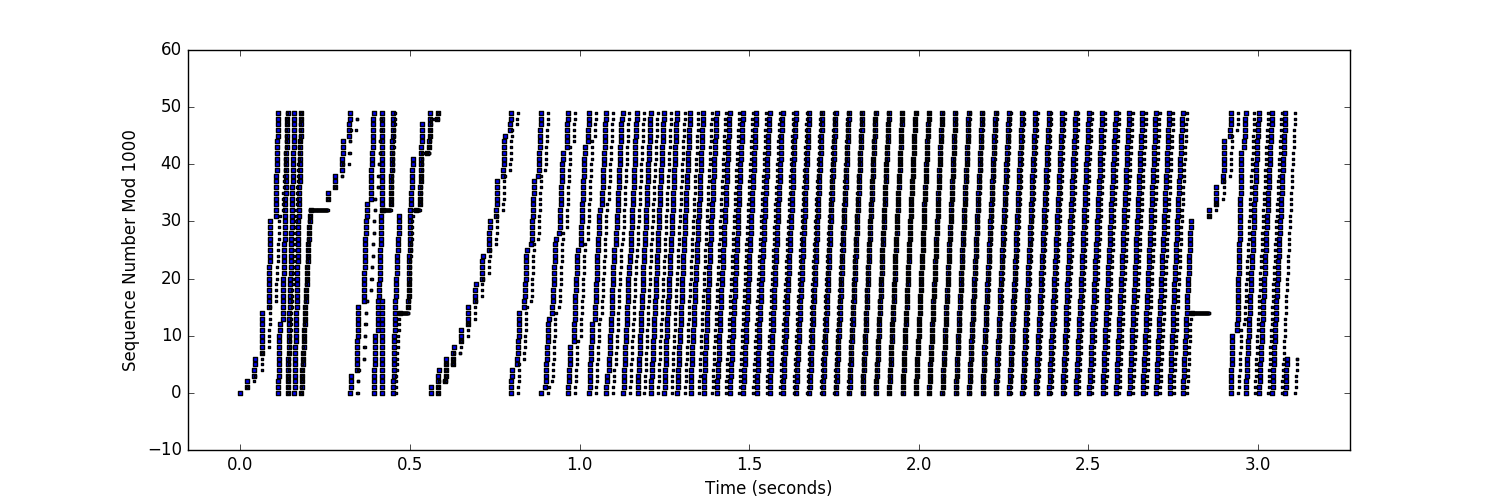
\includegraphics[width=17cm]{charts/one/sequence.png}

\vspace{5mm}

Whenever loss occurs, the window is set back to zero and there's a slow start to the new threshold (Tahoe).

\vspace{5mm}

From the receiver rate, we can see that the one connection uses the entire capacity of the link. It ramps up to full capacity and then appears to ramp down, although we know that it drops off abruptly and the rolling window just makes it appear to be a smooth decent.

\vspace{5mm}

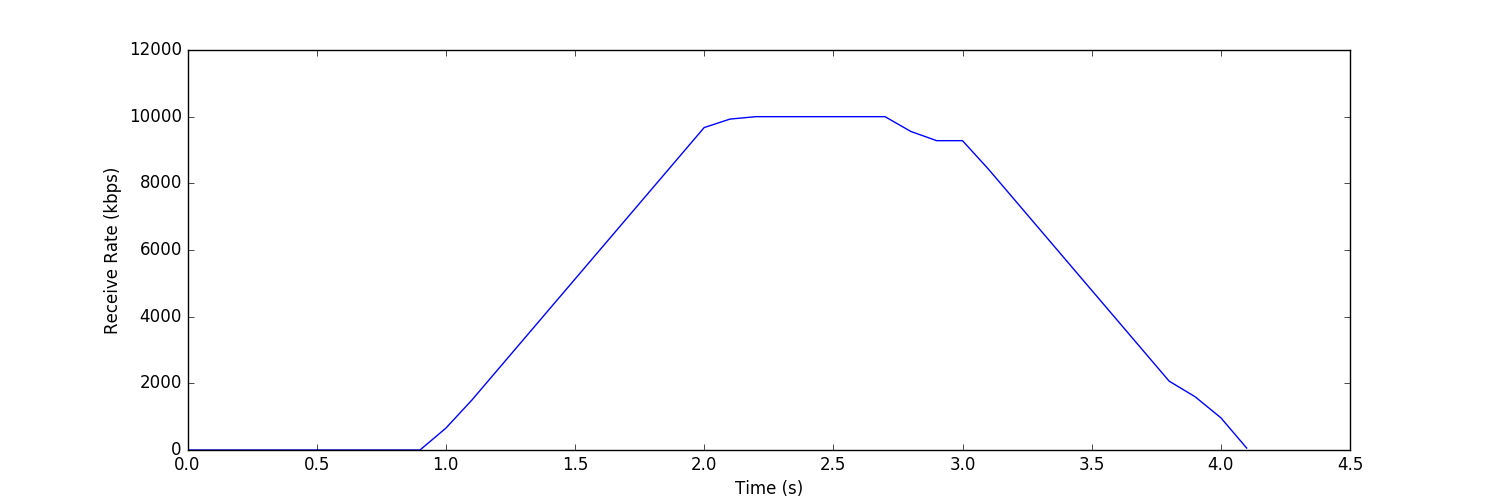
\includegraphics[width=17cm]{charts/one/rateTime1.png}

\vspace{5mm}

The congestion window shows a typical sawtooth pattern. With a larger file or lower queue length we see more "teeth" in the saw, but this diagram is sufficient to show the pattern.

\vspace{5mm}

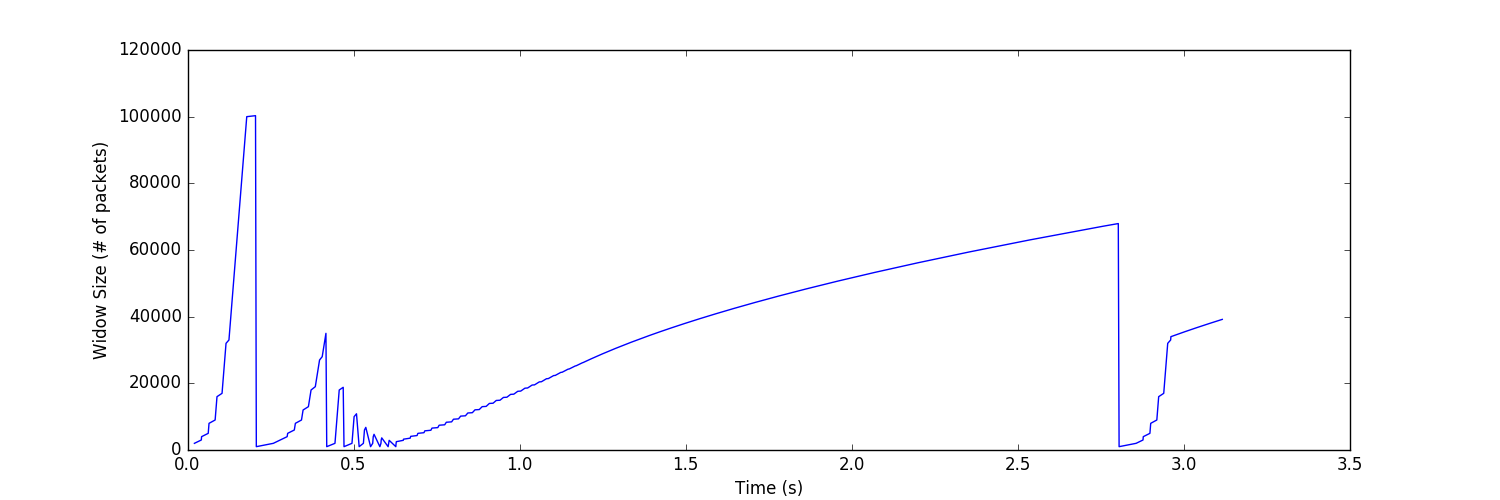
\includegraphics[width=17cm]{charts/one/windowSize1.png}

\vspace{5mm}

The chart of the queue size displays the size of the queue as it grows and the loss (red x's) caused by queue overflow. You can see that it increases quickly at first because of the slow start until there's loss after which it increases at a slower rate.

\vspace{5mm}

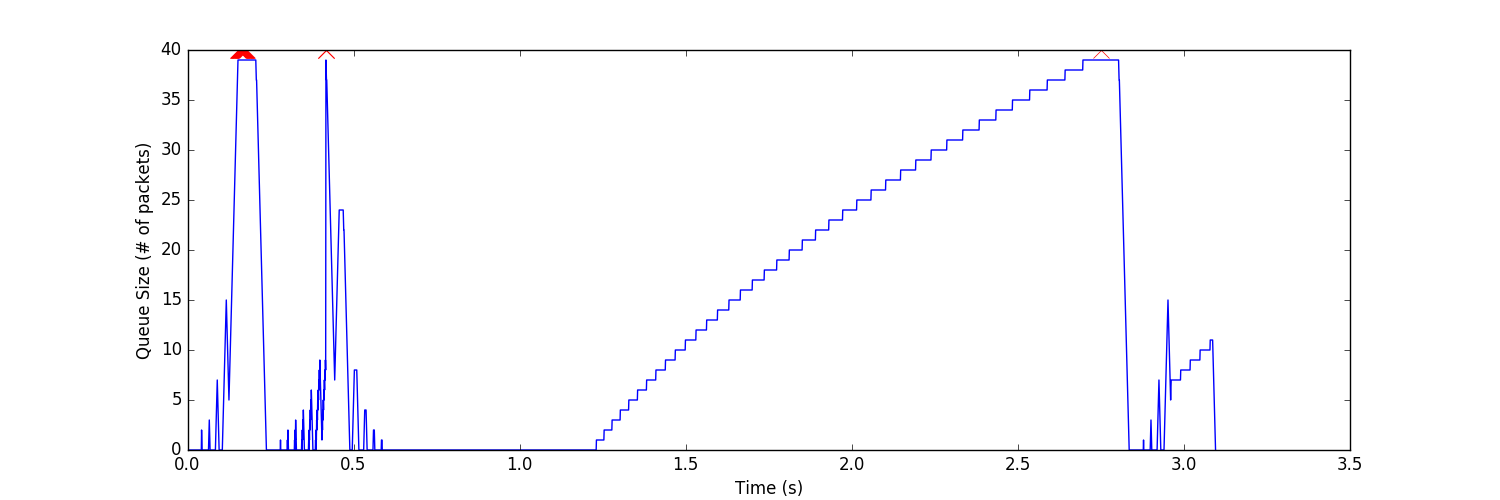
\includegraphics[width=17cm]{charts/one/queueSize.png}

\vspace{5mm}

\subsection{Two Flows}

For the two flow experiment, we added a second pair of connections to send data over. The connection use a copy of test.txt to match the sending of the first link. This connection goes over the exact same path as the first connection.

\vspace{5mm}

\begin{lstlisting}
    c3 = TCP(t1,n1.get_address('n2'),2,n2.get_address('n1'),2,a2,
        window=self.window,threshold=self.threshold,fast_recovery=self.fast_recovery)
    c4 = TCP(t2,n2.get_address('n1'),2,n1.get_address('n2'),2,a2,
        window=self.window,threshold=self.threshold,fast_recovery=self.fast_recovery)
    ...
    with open('test2.txt','r') as f:
        while True:
            data = f.read(1000)
            if not data:
                break
            Sim.scheduler.add(delay=0, event=data, handler=c3.send)
\end{lstlisting}

\vspace{5mm}

The congestion window for the first connection show us a typical sawtooth pattern. It reaches the threshold much more often as the threshold is lower because it's sharing the link with another connection now.

\vspace{5mm}

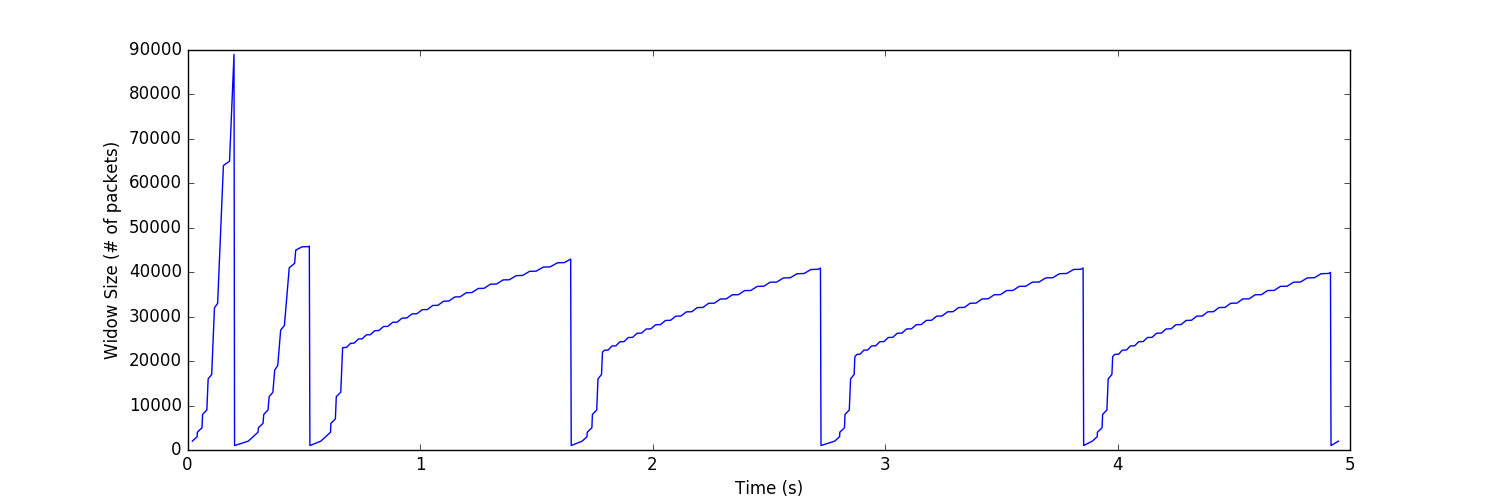
\includegraphics[width=17cm]{charts/two/windowSize1.png}

\vspace{5mm}

The congestion window for the second connection shows us a similar pattern until the first link finishes its transmission, at which point the second connection continues to grow until it finishes its transmission.

\vspace{5mm}

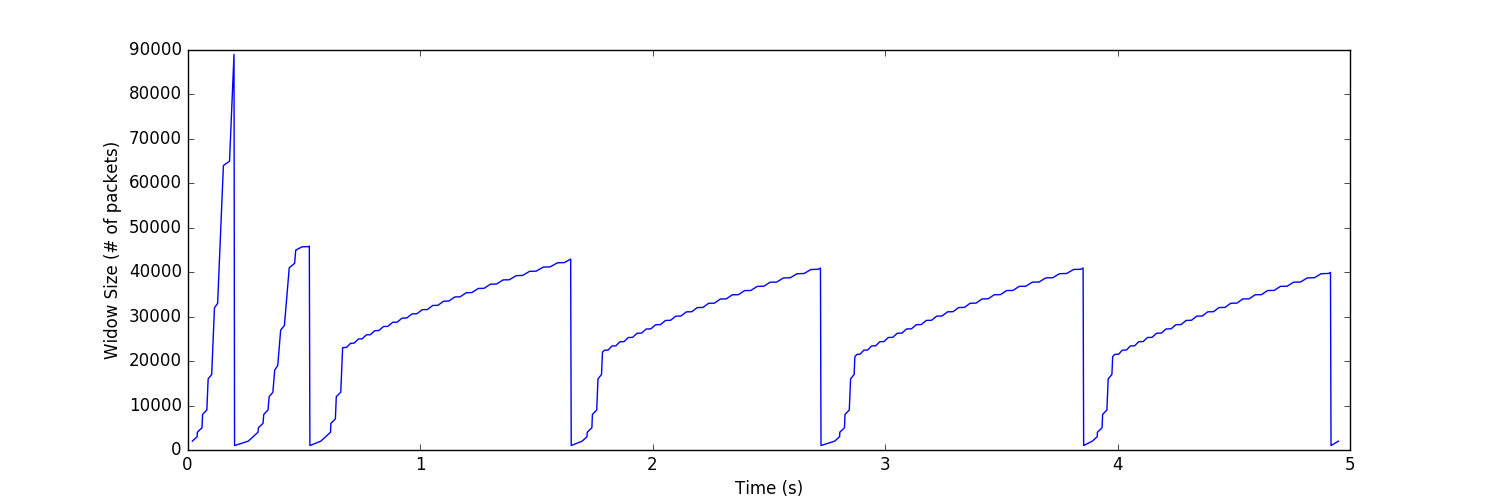
\includegraphics[width=17cm]{charts/two/windowSize1.png}

\vspace{5mm}

The sequence plots for the connections look very similar with slow start at the beginning and then additive increase with resets at the points when there was loss detected.

\vspace{5mm}

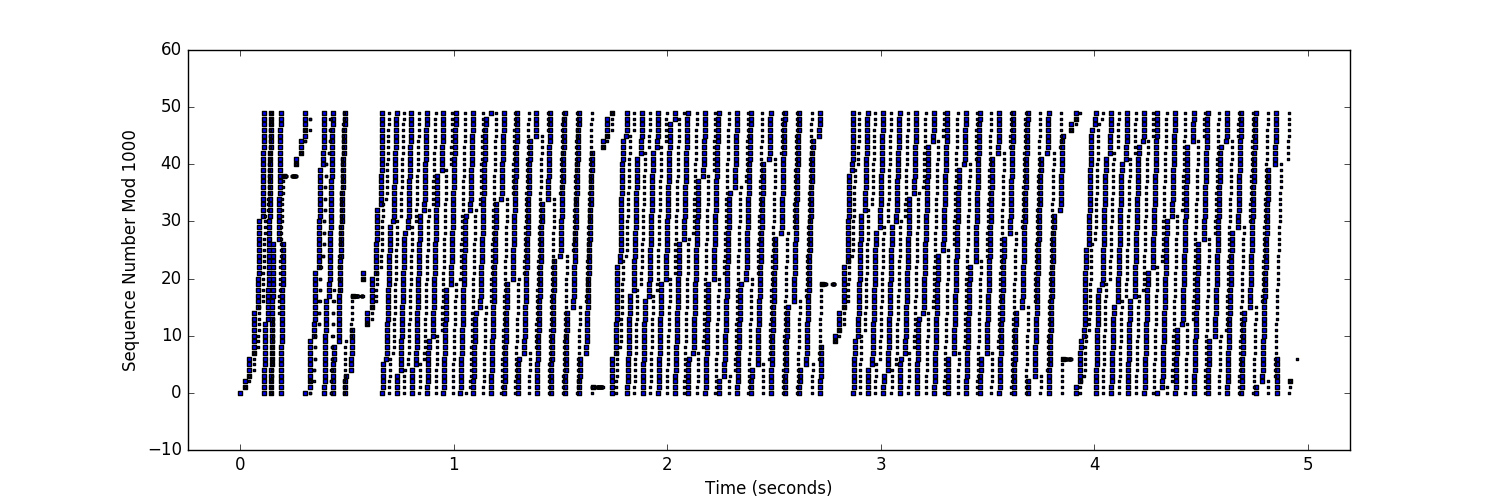
\includegraphics[width=17cm]{charts/two/sequence1.png}

\vspace{5mm}

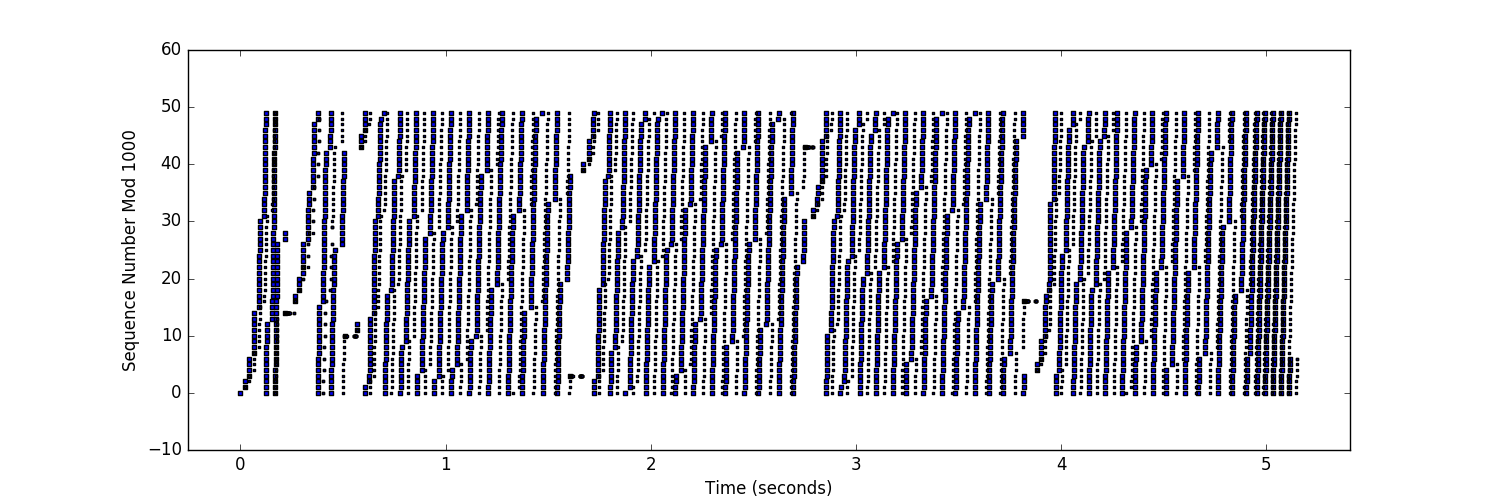
\includegraphics[width=17cm]{charts/two/sequence2.png}

\vspace{5mm}

The visualization of the queue size shows us that the queue grows much more rapidly than with one connection. Packets are lost more often, which causes the connections to reset to 1 MSS window more often.

\vspace{5mm}

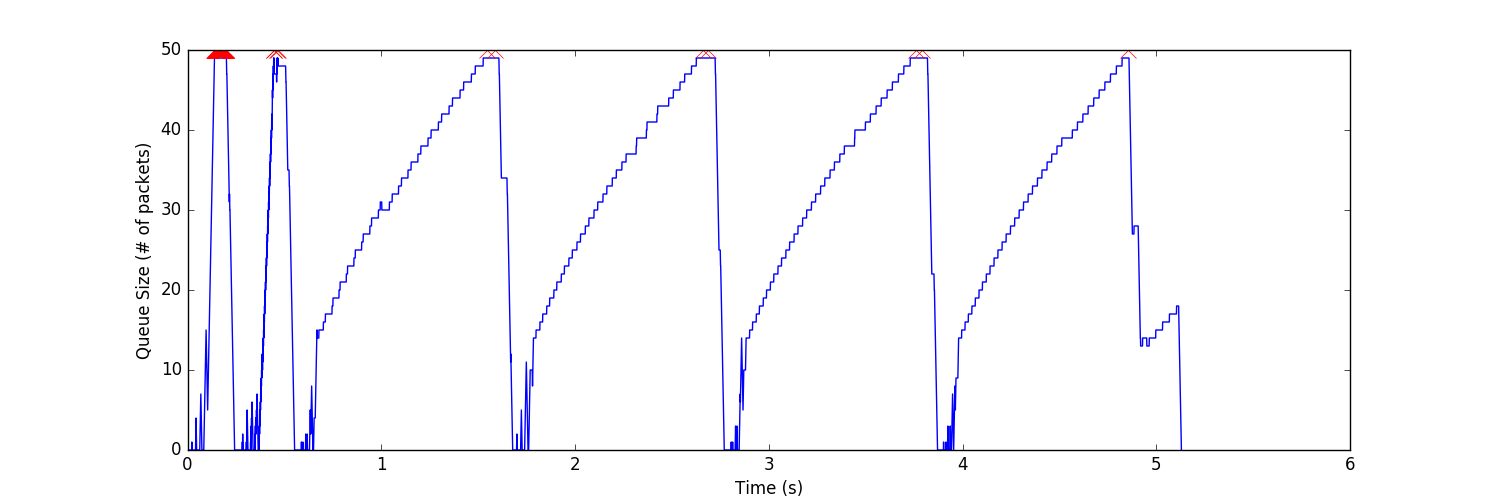
\includegraphics[width=17cm]{charts/two/queueSize.png}

\vspace{5mm}

The receiving rate shows both connections sharing the link. Both connections are oscillating around 1/2 the link capacity.

\vspace{5mm}

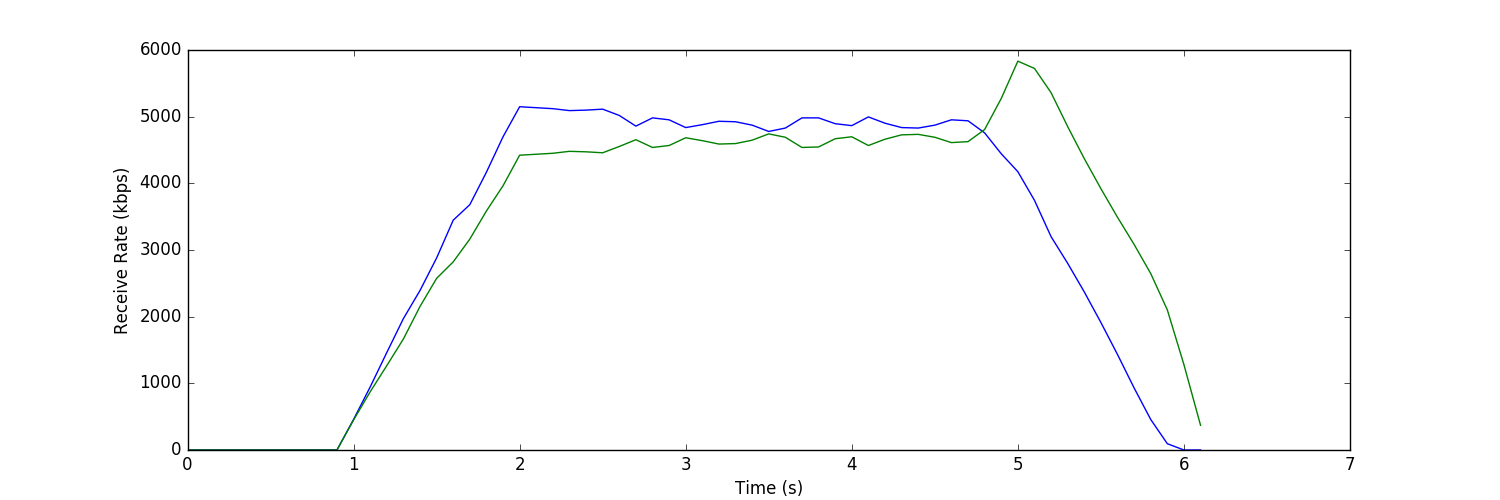
\includegraphics[width=17cm]{charts/two/rateTime.png}

\vspace{5mm}

\subsection{Five Flows}

To get five flows, we multiply the number of files being sent and then number of connections. We offset the file transfers by about 1 second for each connection in order to see the differences clearly. The queue size clearly hits a maximum fairly quickly. The connections cause the queue to grow quickly until there's loss and then they all back off.

\vspace{5mm}

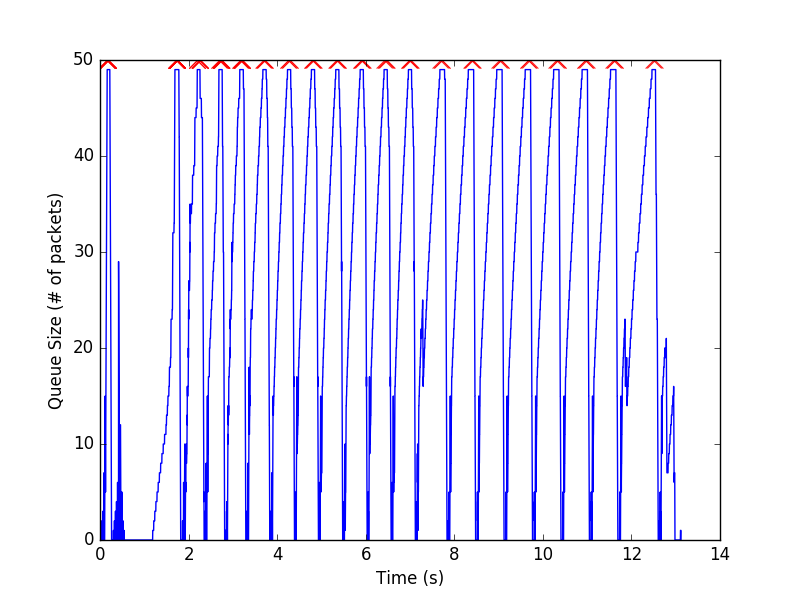
\includegraphics[width=17cm]{charts/five/queueSize.png}

\vspace{5mm}

The receiving rate shows us that as each new connection joins in, the link usage balances out so that each connection gets about 1/n of the link bandwidth (where n is the number of connections).

\vspace{5mm}

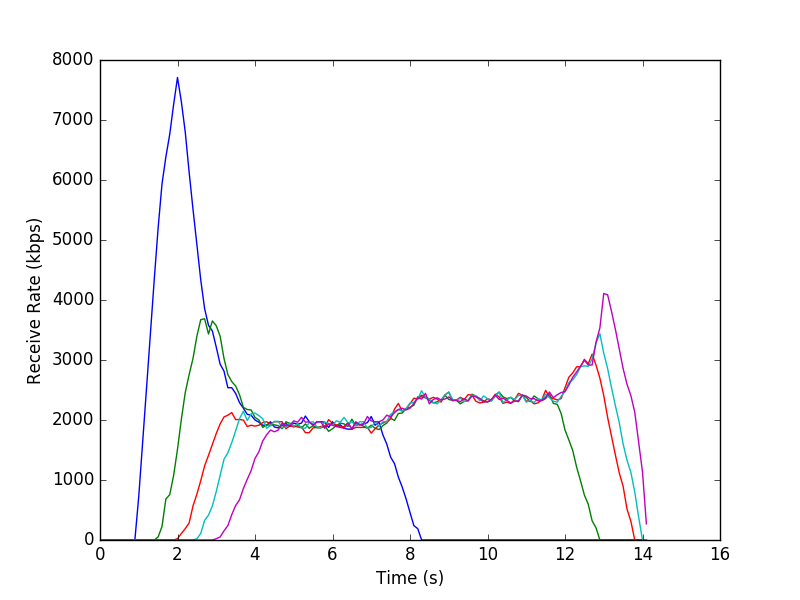
\includegraphics[width=17cm]{charts/five/rateTime5.png}

\vspace{5mm}

\section{Advanced}

\subsection{AIAD}

In this experiment we used additive increase, additive decrease. Instead of decreasing the window size back to 1 MSS when there was loss or even dividing the window in half, we just subtracted 1 MSS from the current window size.

\vspace{5mm}

\begin{lstlisting}
    # if the AIAD setting is turned on
    if self.aiad:
        self.window -= self.mss
        self.state = 1
\end{lstlisting}

\vspace{5mm}

We noticed that this caused many more losses in the queue over time. The queue oscillated between empty and full as the sending rate changed. Eventually, the queue size seemed to even out and oscillated from 0 to around 10. This was caused by the round trip time adjustments.

\vspace{5mm}

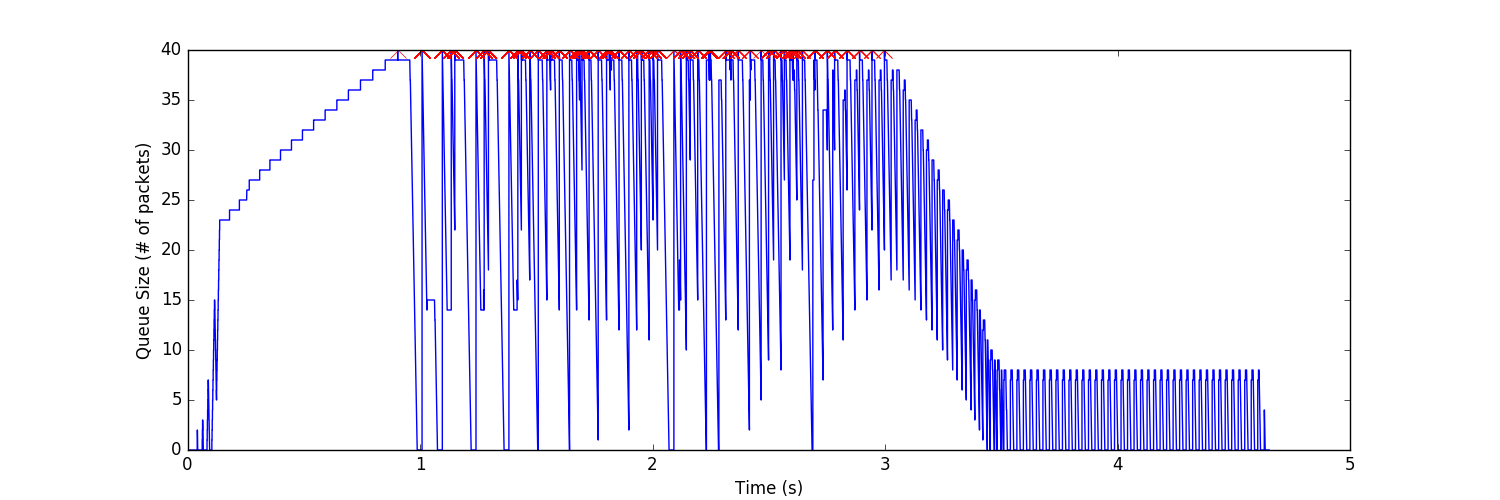
\includegraphics[width=17cm]{charts/advanced/aiad/queueSize.png}

\vspace{5mm}

The throughput seemed to stay relatively constant. The rate climed to link capacity and stayed there until the packet finished transmitting. However, the rate didn't drop off as steeply at the end which leads to believe that many packets had to be retransmitted because of loss.

\vspace{5mm}

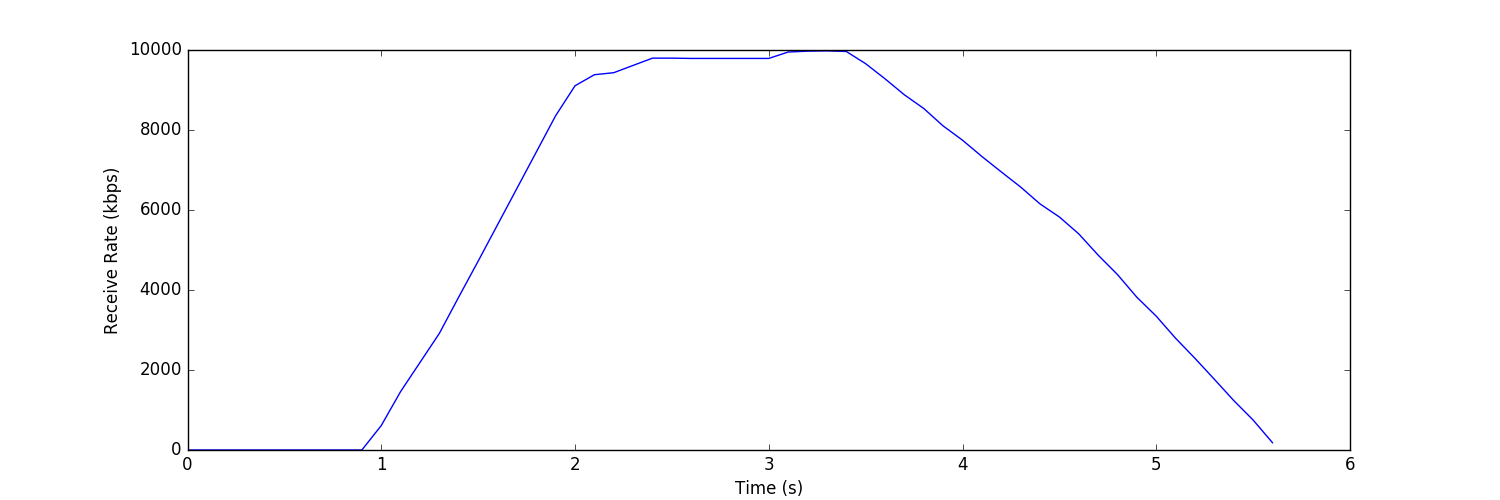
\includegraphics[width=17cm]{charts/advanced/aiad/rateTime1.png}

\vspace{5mm}

The change in window size leads to an interesting discussion. The slow start takes the window to well over the link capacity and it has to scale back. However, because the decrease was only additive, the window size takes a long time to decrease to a sufficient point to where it's stable.

\vspace{5mm}

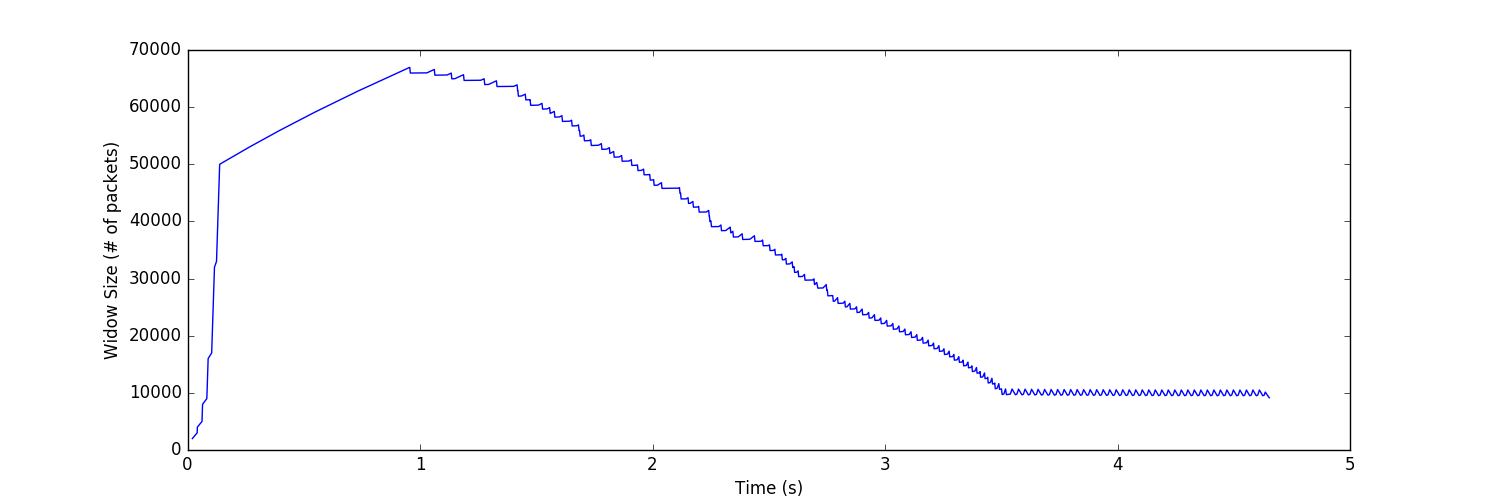
\includegraphics[width=17cm]{charts/advanced/aiad/windowSize1.png}

\vspace{5mm}

From these findings, it would appear that TCP is still stable with only one connection under AIAD circumstances, however much more loss was experienced.

\subsection{AIMD}

In this experiment, we set up one connection but had it decrease at a slower rate than normal (5/6 instead of 1/2). We used fast recovery to make sure the changes were easily observable. We created an additive increase, multiplicative decrease constant (AIMDC) that could be configured per connection. The default was 0.5.

\vspace{5mm}

\begin{lstlisting}
    # AIMD Constant
    self.aimdc = aimdc
\end{lstlisting}

\vspace{5mm}

The first difference we noticed was in the queue size. The queue grew to capacity as before but as it decreased it oscillated at a low queue length until it finished.

\vspace{5mm}

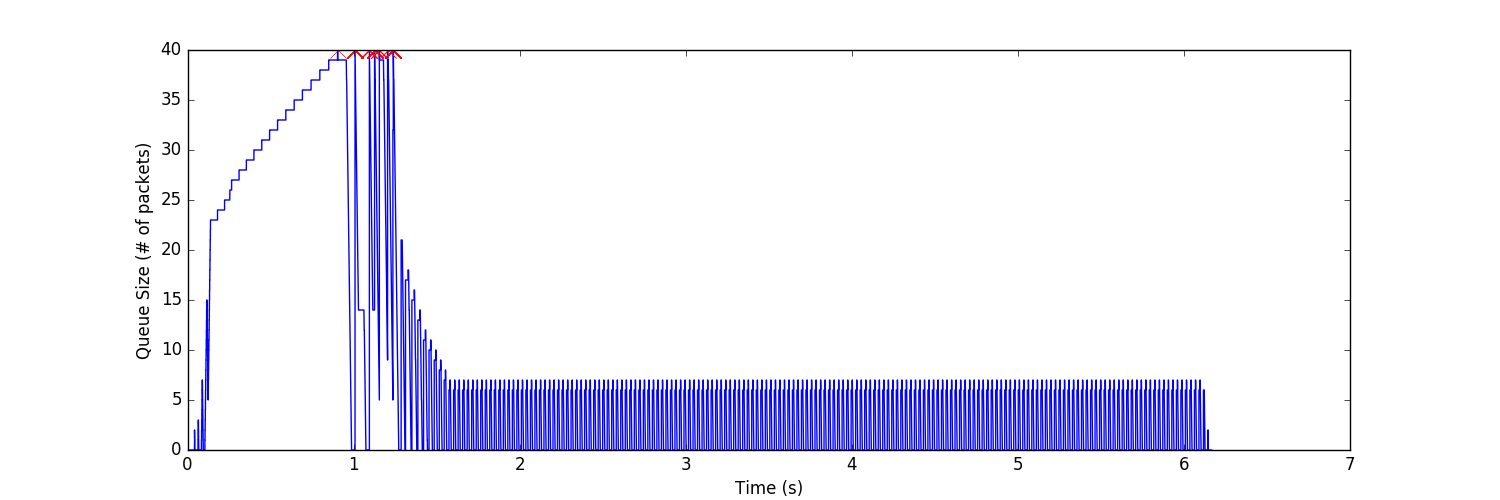
\includegraphics[width=17cm]{charts/advanced/aimd/queueSize.png}

\vspace{5mm}

The rate peaks and then levels off at about half of the link capacity. We're not sure what causes this, but it appears that the queue length keeps it from growing to the full link capacity.

\vspace{5mm}

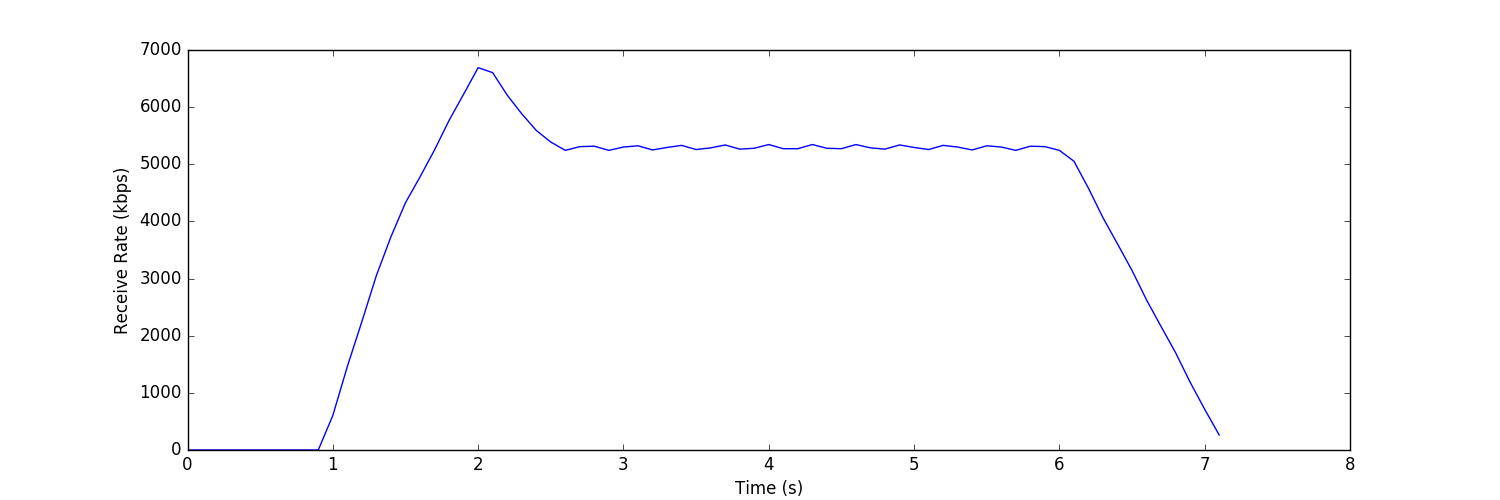
\includegraphics[width=17cm]{charts/advanced/aimd/rateTime1.png}

\vspace{5mm}

The window grows quickly at first and has to experience multiple losses before it gets down to a steady rate.

\vspace{5mm}

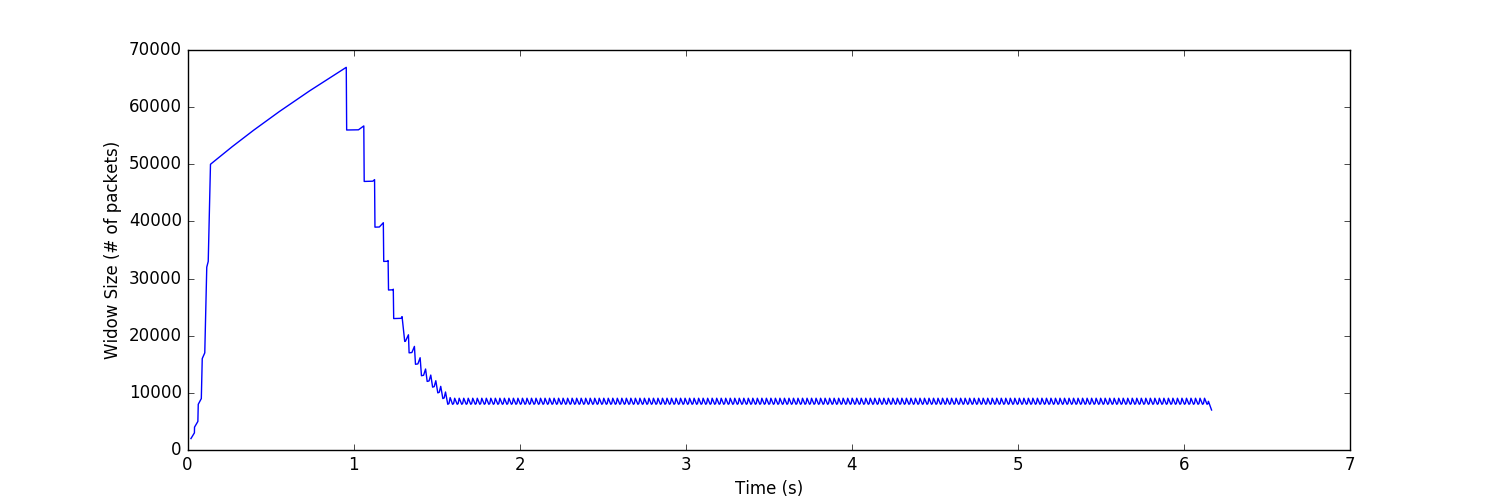
\includegraphics[width=17cm]{charts/advanced/aimd/windowSize1.png}

\vspace{5mm}

From these results, we concluded that AIMD with a higher multiplicative constant is still stable although it may not be optimal.

\subsection{Competing AIMD}

In this experiment, we had two connections. One had the normal multiplicative constant of 1/2 and the other had a higher multiplicative constant of 5/6. We asked if they would still get an equal share of the bandwidth. Taking a look at the receiving rate, it appears that the link with a higher multiplicative constant took a much larger share of the bandwidth. That link took roughly 2/3 of the capacity while the other link took about 1/3. After one link finishes transmitting, the other link takes the remainder of the bandwidth.

\vspace{5mm}

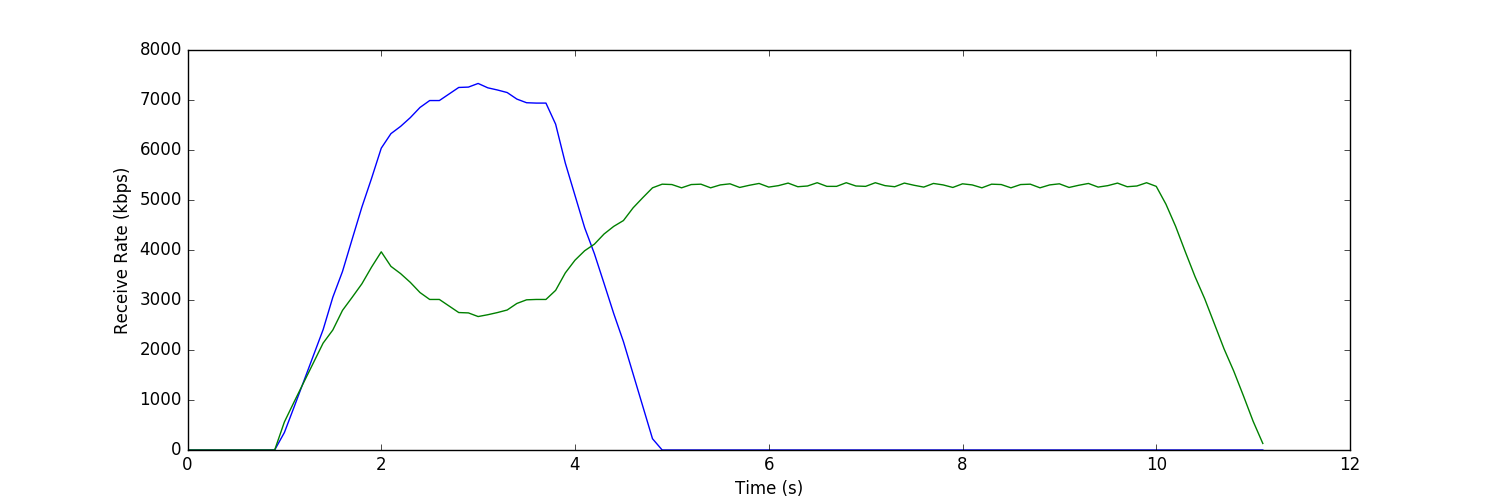
\includegraphics[width=17cm]{charts/advanced/competingAimd/rateTime.png}

\vspace{5mm}

We can see from the window size of the link with the larger multiplicative constant that it retains a higher sending rate for longer.

\vspace{5mm}

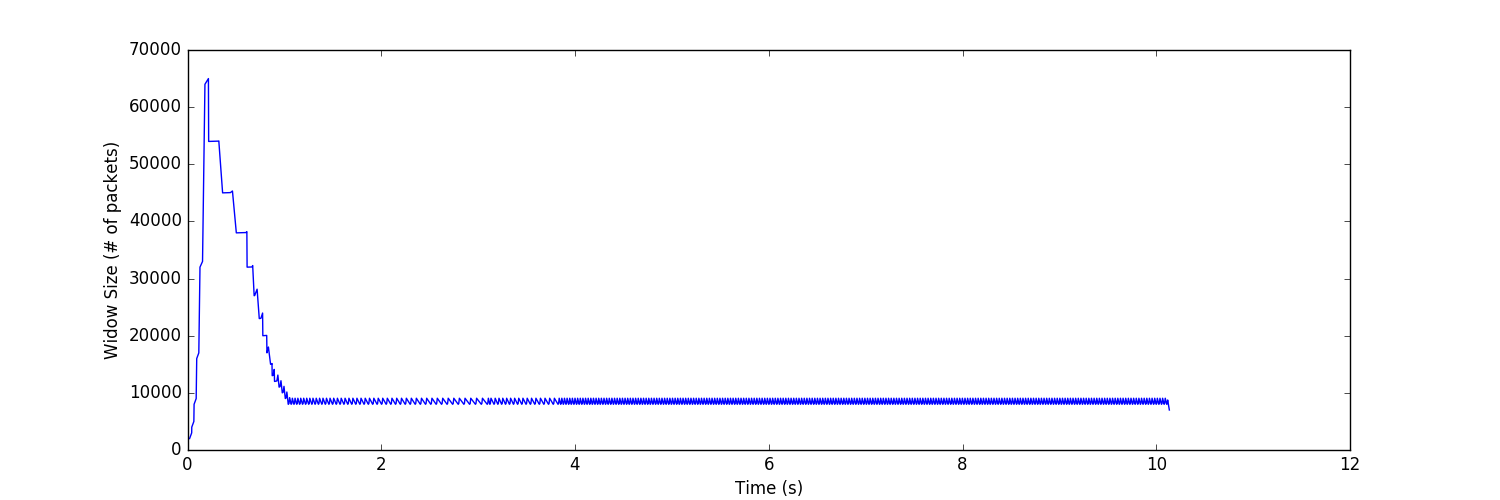
\includegraphics[width=17cm]{charts/advanced/competingAimd/windowSize2.png}

\vspace{5mm}

The other link has a "normal" looking sawtooth pattern.

\vspace{5mm}

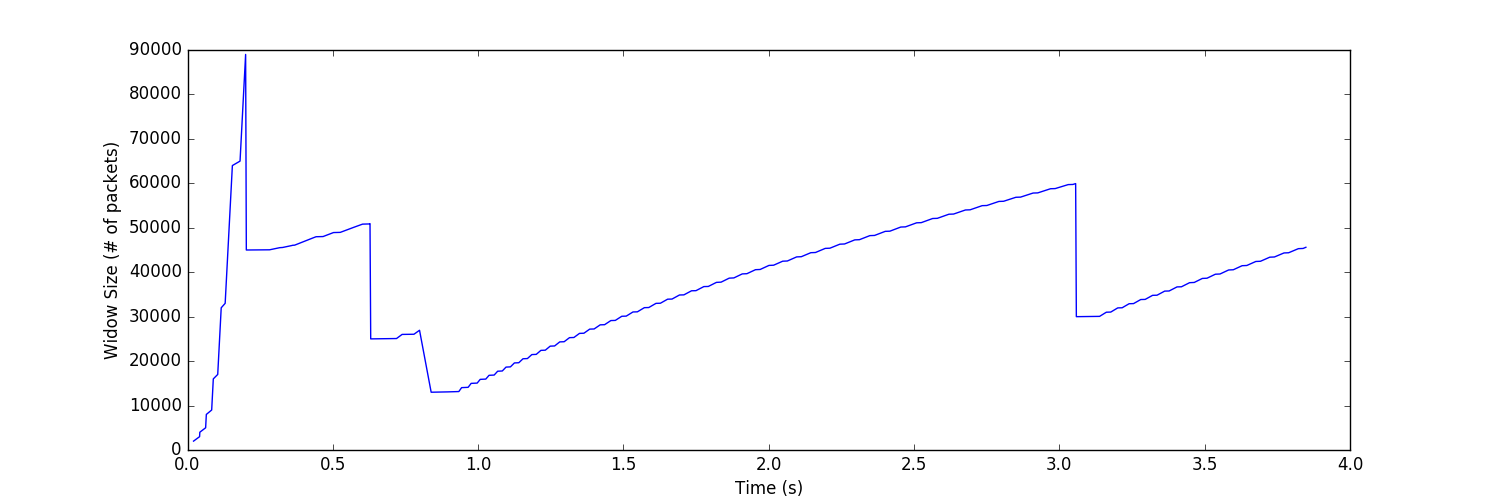
\includegraphics[width=17cm]{charts/advanced/competingAimd/windowSize1.png}

\vspace{5mm}

From these charts we concluded that a link with a higher multiplicative constant will take a larger portion of the link bandwidth.

\subsection{Competing RTT}

In this experiment, we set up two connections using 4 nodes. The first two nodes, n1 and n2 branched into n3 which connected to n4.

\vspace{5mm}

\begin{lstlisting}
    # setup routes
    # n1 - n3 - n4
    #      |
    #     n2
    n1 = net.get_node('n1')
    n2 = net.get_node('n2')
    n3 = net.get_node('n3')
    n4 = net.get_node('n4')
\end{lstlisting}

\vspace{5mm}

In the network configuration we set the propagation delay on the link between n1 and n3 to 100ms and the propagation delay on all other links to 10ms.

\vspace{5mm}

\begin{lstlisting}
    #
    n1 n3
    n2 n3
    n3 n1 n2 n4
    n4 n3

    # link configuration
    n1 n3 100pkts 10Mbps 100ms
    n3 n1 100pkts 10Mbps 100ms

    n2 n3 100pkts 10Mbps 10ms
    n3 n2 100pkts 10Mbps 10ms

    n3 n4 100pkts 10Mbps 10ms
    n4 n3 100pkts 10Mbps 10ms
\end{lstlisting}

\vspace{5mm}

We connected the network so that n1 and n3 were linked, n2 and n3 were linked, and n3 and n4 were linked.

\vspace{5mm}

\begin{lstlisting}
    # n1 forwarding entries
    n1.add_forwarding_entry(address=n3.get_address('n1'),link=n1.links[0])
    n1.add_forwarding_entry(address=n4.get_address('n3'),link=n1.links[0])

    # n2 forwarding entries
    n2.add_forwarding_entry(address=n3.get_address('n2'),link=n2.links[0])
    n2.add_forwarding_entry(address=n4.get_address('n3'),link=n2.links[0])

    # n3 forwarding entries
    n3.add_forwarding_entry(address=n1.get_address('n3'),link=n3.links[0])
    n3.add_forwarding_entry(address=n2.get_address('n3'),link=n3.links[1])
    n3.add_forwarding_entry(address=n4.get_address('n3'),link=n3.links[2])

    # n4 forwarding entries
    n4.add_forwarding_entry(address=n1.get_address('n3'),link=n4.links[0])
    n4.add_forwarding_entry(address=n2.get_address('n3'),link=n4.links[0])
    n4.add_forwarding_entry(address=n3.get_address('n4'),link=n4.links[0])
\end{lstlisting}

\vspace{5mm}

This allowed us to set up connections from n1 to n4 with 110 ms propagation delay and from n2 to n4 with 20 ms propagation delay.

\vspace{5mm}

\begin{lstlisting}
    # setup connection
    c1 = TCP(t1,n1.get_address('n3'),1,n4.get_address('n3'),1,a1)
    c2 = TCP(t4,n4.get_address('n3'),1,n1.get_address('n3'),1,a1)

    c3 = TCP(t2,n2.get_address('n3'),2,n4.get_address('n3'),2,a2)
    c4 = TCP(t4,n4.get_address('n3'),2,n2.get_address('n3'),2,a2)
\end{lstlisting}

\vspace{5mm}

We wanted to know if the links would get equal shares of the bandwidth. The receiving rate graph shows that the link with the smaller propagation delay gets a much higher percentage of the link bandwidth.

\vspace{5mm}

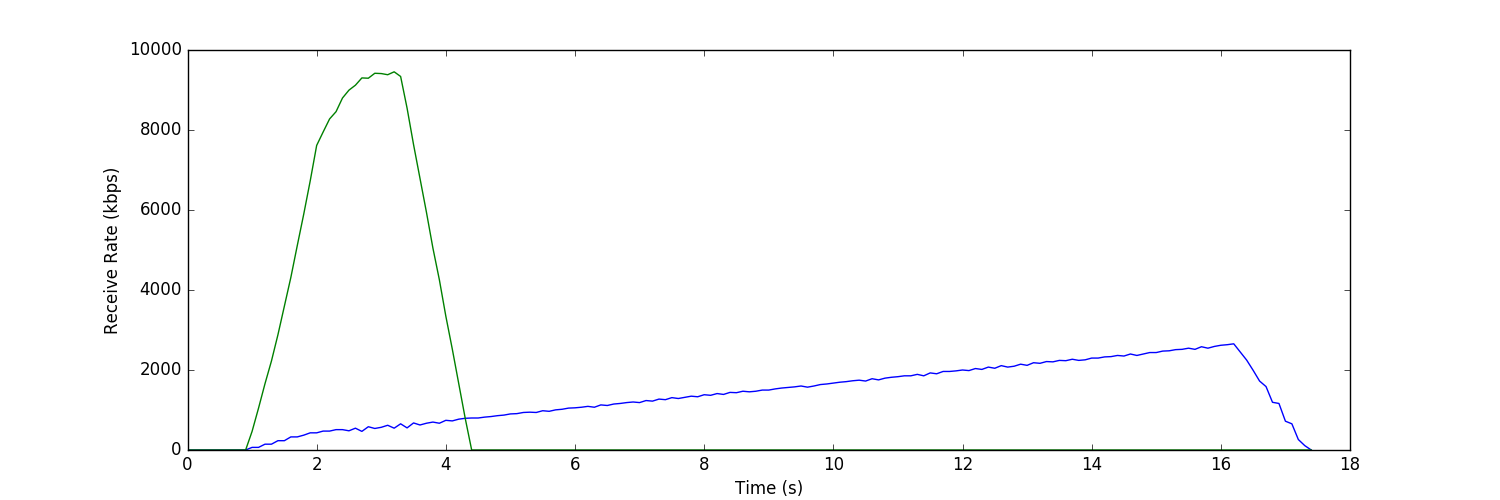
\includegraphics[width=17cm]{charts/advanced/competingRtt/rateTime.png}

\vspace{5mm}

This happens because the lower delay allows the link to receive ACKs quicker and increase its window size at a quicker rate.

\vspace{5mm}

\vspace{5mm}

\end{document}
